\documentclass[11pt]{article}

%%%%%%%%%%%%%%%%%%%%%%%%%%%%%%%%%%%%%%%%%%%%%%%%%%%%%%%%%%%%%%%
%                      Customize Header                       %
%%%%%%%%%%%%%%%%%%%%%%%%%%%%%%%%%%%%%%%%%%%%%%%%%%%%%%%%%%%%%%%

\newcommand{\assessmentTitle}{
CheckIt Assessment
}
\newcommand{\assessmentVersion}{
Version 1777691306914
}
\newcommand{\assessmentInstructions}{
Do not use any unapproved aids while taking this assessment.
Read each question carefully and be sure to show all work
in the space provided.
}

%%%%%%%%%%%%%%%%%%%%%%%%%%%%%%%%%%%%%%%%%%%%%%%%%%%%%%%%%%%%%%%
%%%%%%%%%%%%%%%%%%%%%%%%%%%%%%%%%%%%%%%%%%%%%%%%%%%%%%%%%%%%%%%



\usepackage{amsfonts,amssymb,amsmath,amsthm}
\setcounter{MaxMatrixCols}{50}
\usepackage{hyperref}
\let\oldhref\href\renewcommand{\href}[2]{\oldhref{#1}{#2}\footnote{\url{#1}}}
\usepackage[margin=1in,tmargin=2in,headheight=84pt]{geometry}
\usepackage{enumerate}
\usepackage{graphicx}
\usepackage{fancyhdr}
\usepackage{lastpage}
\pagestyle{fancy}
\fancyhf{}
\rhead{Name: \underline{\hspace{2.5in}}\\ID: \underline{\hspace{2.5in}}

\vspace{2.5em}}
\chead{\vspace{2.5em}

\fbox{\fbox{\parbox{6in}{\centering\assessmentInstructions}}}}
\lhead{\assessmentTitle \hspace{2em} \assessmentVersion

\vspace{2.5em}}
\rfoot{Page \thepage\ of \pageref{LastPage}}
\setlength{\headheight}{80pt}
\renewcommand{\headrulewidth}{0pt}


\begin{document}

\begin{enumerate}

% 

\item %%%%% SpaTeXt Commands %%%%%
\providecommand{\stxKnowl}{}\renewcommand{\stxKnowl}[1]{#1}
\providecommand{\stxOuttro}{}\renewcommand{\stxOuttro}[1]{#1}
\providecommand{\stxTitle}{}\renewcommand{\stxTitle}[1]{#1}
% Comment next line to show outtros
\renewcommand{\stxOuttro}[1]{}
%%%%%%%%%%%%%%%%%%%%%%%%%%%%
\stxKnowl{
 Evaluate the difference quotient, \(\displaystyle{ \frac{f(x+h)-f(x)}{h}}\) , for \(f(x) = x^{2} + 1\). 

\stxOuttro{
SOLUTION

 \(f(x+h) = 1(x+h)^2 + 1\) 

 \(= 1(x^2 + 2xh + h^2) + 1\) 

 \(= h^{2} + 2 \, h x + x^{2} + 1\) 

 \(\displaystyle{\frac{f(x+h)-f(x)}{h} = \frac{ (h^{2} + 2 \, h x + x^{2} + 1) - (x^{2} + 1) }{h}}\) 

 \(=\displaystyle{ \frac{ h^{2} + 2 \, h x }{h}}\) 

 \(= \displaystyle{ \frac{ h(h + 2 \, x) }{h}}\) 

 \(\boxed{ h + 2 \, x }\) 

}
}

\newpage

% 

\item %%%%% SpaTeXt Commands %%%%%
\providecommand{\stxKnowl}{}\renewcommand{\stxKnowl}[1]{#1}
\providecommand{\stxOuttro}{}\renewcommand{\stxOuttro}[1]{#1}
\providecommand{\stxTitle}{}\renewcommand{\stxTitle}[1]{#1}
% Comment next line to show outtros
\renewcommand{\stxOuttro}[1]{}
%%%%%%%%%%%%%%%%%%%%%%%%%%%%
\stxKnowl{
 Use the table to identify the transformations of the toolkit function described by the equation. Circle the option that applies and fill in the blanks as appropriate to describe the transformations of the given function. If one does not apply, you may leave it blank. Then sketch the transformed graph, indicating any asymptotes with dashed lines, and state the resulting domain and range. 

\(f(x) = \log_{2}(x + 3) + 7\)

 \[\begin{array}{|l|l|} \hline \rule[-0.8em]{0pt}{2.2em} \textbf{Horizontal Transformations} & \textbf{Vertical Transformations} \\ \hline \rule[-1.2em]{0pt}{3em} \text{Reflection: YES or NO} & \text{Reflection: YES or NO} \\ \hline \rule[-1.2em]{0pt}{3em} \text{Dilation: \underline{\hspace{2cm}} times as wide} & \text{Dilation: \underline{\hspace{2cm}} times as tall} \\ \hline \rule[-1.2em]{0pt}{3em} \text{Translation: \underline{\hspace{2cm}} units LEFT or RIGHT} & \text{Translation: \underline{\hspace{2cm}} units UP or DOWN} \\ \hline \end{array}\] 

 \[\begin{tikzpicture}[scale=0.39,>=triangle 45] \draw[step=1cm, black!60] (-10,-10) grid (10,10); \draw[very thick, <->] (-10.5,0) -- (10.5,0); \draw[very thick, <->] (0,-10.5) -- (0,10.5); \end{tikzpicture}\] 

\stxOuttro{
SOLUTION



\begin{itemize}
\item
 \(\textbf{Horizontal: } \text{Reflection: NO, Dilation: 1, Shift: 3 units LEFT.}\) 

\item
 \(\textbf{Vertical: } \text{Reflection: NO, Dilation: 1, Shift: 7 units UP.}\) 

\end{itemize}


 \[\begin{tikzpicture}[scale=0.39,>=triangle 45] \draw[step=1cm, black!60] (-10,-10) grid (10,10); \draw[very thick, <->] (-10.5,0) -- (10.5,0); \draw[very thick, <->] (0,-10.5) -- (0,10.5); \clip (-10.5,-10.5) rectangle (10.5,10.5);\draw[dashed, red, thick] (-3, -10.5) -- (-3, 10.5);\draw[blue, very thick, samples=100, domain=-2.99000000000000:10.5000000000000, smooth] plot (\x, {(ln(\x - (-3))/ln(2)) + (7)});\end{tikzpicture}\] 



\begin{itemize}
\item
 \(\textbf{Domain: } (-3, \infty)\) 

\item
 \(\textbf{Range: } (-\infty, \infty)\) 

\end{itemize}
}
}

\newpage

% 

\item %%%%% SpaTeXt Commands %%%%%
\providecommand{\stxKnowl}{}\renewcommand{\stxKnowl}[1]{#1}
\providecommand{\stxOuttro}{}\renewcommand{\stxOuttro}[1]{#1}
\providecommand{\stxTitle}{}\renewcommand{\stxTitle}[1]{#1}
% Comment next line to show outtros
\renewcommand{\stxOuttro}[1]{}
%%%%%%%%%%%%%%%%%%%%%%%%%%%%
\stxKnowl{
Solve each of the following equations. Give exact solutions.

\begin{enumerate}
\item
\stxKnowl{
\(5^{-4 \, x} \cdot 5^{3 \, x} = 5\)

\stxOuttro{
\(\begin{aligned} 5^{-4 \, x+3 \, x} &= 5 \\ -4 \, x+3 \, x &= 1 \\ -x &= 1 \\ x &= -1 \end{aligned}\)

\(\boxed{x = -1}\)

}
}

\item
\stxKnowl{
\(\log_{3}(x + 1) + \log_{3}(x - 1) = 1\)

\stxOuttro{
\(\begin{aligned} \log_{3}((x + 1)(x - 1)) &= 1 \\ 3 &= (x + 1)(x - 1) \\ 3 &= x^{2} - 1 \\ 0 &= x^{2} - 4 \\ 0 &= (x - 2)(x + 2) \end{aligned}\)

\(\boxed{x = 2} \quad \text{(Extraneous: } x = -2 \text{)}\)

}
}

\end{enumerate}
}

\newpage

% 

\item %%%%% SpaTeXt Commands %%%%%
\providecommand{\stxKnowl}{}\renewcommand{\stxKnowl}[1]{#1}
\providecommand{\stxOuttro}{}\renewcommand{\stxOuttro}[1]{#1}
\providecommand{\stxTitle}{}\renewcommand{\stxTitle}[1]{#1}
% Comment next line to show outtros
\renewcommand{\stxOuttro}[1]{}
%%%%%%%%%%%%%%%%%%%%%%%%%%%%
\stxKnowl{
Use logarithm identities to determine the exact value of the expression, given \(\log_b(m)=9\), \(\log_b(n-1)=8\), and \(\log_b(p)=4\).

\(\log_b\left(\frac{m\sqrt[4]{n-1}}{p^{4}}\right)\)

\stxOuttro{
\(9 + \frac{1}{4}(8) - 4(4)\)

\(9 + 2 - 16\)

\(\boxed{-5}\)

}
}

\newpage

% 

\item %%%%% SpaTeXt Commands %%%%%
\providecommand{\stxKnowl}{}\renewcommand{\stxKnowl}[1]{#1}
\providecommand{\stxOuttro}{}\renewcommand{\stxOuttro}[1]{#1}
\providecommand{\stxTitle}{}\renewcommand{\stxTitle}[1]{#1}
% Comment next line to show outtros
\renewcommand{\stxOuttro}[1]{}
%%%%%%%%%%%%%%%%%%%%%%%%%%%%
\stxKnowl{
Given the information below, solve the right triangle for all missing sides and angles.

Triangle \(ABC\) satisfies \(\angle A = 29.7^\circ\), \(\angle C = 90^\circ\), and \(b = 44\).

Round side lengths to the nearest hundredth and angles to the nearest tenth of a degree.

\stxOuttro{
\(B = 90^\circ - 29.7^\circ = 60.3^\circ\)

\(\tan(29.7^\circ) = \frac{a}{44} \implies a = 44\tan(29.7^\circ) \approx 25.10\)

\(\cos(29.7^\circ) = \frac{44}{c} \implies c = \frac{44}{\cos(29.7^\circ)} \approx 50.65\)

\(\boxed{\begin{aligned} A &= 29.7^\circ & a &\approx 25.10 \\ B &= 60.3^\circ & b &\approx 44.00 \\ C &= 90^\circ & c &\approx 50.65 \end{aligned}}\)

}
}

\newpage

% 

\item %%%%% SpaTeXt Commands %%%%%
\providecommand{\stxKnowl}{}\renewcommand{\stxKnowl}[1]{#1}
\providecommand{\stxOuttro}{}\renewcommand{\stxOuttro}[1]{#1}
\providecommand{\stxTitle}{}\renewcommand{\stxTitle}[1]{#1}
% Comment next line to show outtros
\renewcommand{\stxOuttro}[1]{}
%%%%%%%%%%%%%%%%%%%%%%%%%%%%
\stxKnowl{
Verify the given identity.

\[\frac{\cos^2(\alpha) - \sin^2(\alpha)}{2\sin(\alpha)\cos(\alpha)} = \cot(2\alpha)\]

\stxOuttro{
\(\frac{\cos^2(\alpha) - \sin^2(\alpha)}{2\sin(\alpha)\cos(\alpha)}\)

\(= \frac{\cos(2\alpha)}{\sin(2\alpha)}\)

\(= \boxed{\cot(2\alpha)}\)

}
}

\newpage

% 

\item %%%%% SpaTeXt Commands %%%%%
\providecommand{\stxKnowl}{}\renewcommand{\stxKnowl}[1]{#1}
\providecommand{\stxOuttro}{}\renewcommand{\stxOuttro}[1]{#1}
\providecommand{\stxTitle}{}\renewcommand{\stxTitle}[1]{#1}
% Comment next line to show outtros
\renewcommand{\stxOuttro}[1]{}
%%%%%%%%%%%%%%%%%%%%%%%%%%%%
\stxKnowl{
Find all solutions on the interval \([0^\circ, 360^\circ)\). Round approximate solutions to the nearest tenth of a degree as appropriate.

\[3 \cos \theta = -2\]

\stxOuttro{
\(\cos \theta = -\frac{2}{3}\)

\(\theta = \cos^{-1}\left(-\frac{2}{3}\right)\)

\(\theta \approx 131.8103^\circ \dots\)

\(360^\circ - 131.8103^\circ \approx 228.1897^\circ\)

\(\boxed{\theta = 131.8^\circ, 228.2^\circ}\)

}
}

\newpage

% 

\item %%%%% SpaTeXt Commands %%%%%
\providecommand{\stxKnowl}{}\renewcommand{\stxKnowl}[1]{#1}
\providecommand{\stxOuttro}{}\renewcommand{\stxOuttro}[1]{#1}
\providecommand{\stxTitle}{}\renewcommand{\stxTitle}[1]{#1}
% Comment next line to show outtros
\renewcommand{\stxOuttro}[1]{}
%%%%%%%%%%%%%%%%%%%%%%%%%%%%
\stxKnowl{
Given the information below, solve the triangle. If more than one triangle is possible, find \textbf{all} solutions.

Triangle \(ABC\) satisfies \(\angle A = 29^\circ\), \(a = 6.9\), and \(b = 11.4\).

Round sides to the nearest hundredth and angles to the nearest tenth of a degree.

\stxOuttro{
\(\frac{\sin(B)}{b} = \frac{\sin(A)}{a}\)

\(\sin(B) = \frac{11.4\sin(29^\circ)}{6.9} \approx 0.8010\)

\(B_1 = \sin^{-1}(0.8010) \approx 53.2^\circ\)

\(B_2 = 180^\circ - 53.2^\circ = 126.8^\circ\)

\(29^\circ + 126.8^\circ = 155.8^\circ < 180^\circ\)

\(C_1 = 180^\circ - 29^\circ - 53.2^\circ = 97.8^\circ\)

\(c_1 = \frac{a\sin(C_1)}{\sin(A)}\)

\(c_1 = \frac{6.9\sin(97.8^\circ)}{\sin(29^\circ)} \approx 14.10\)

\(C_2 = 180^\circ - 29^\circ - 126.8^\circ = 24.2^\circ\)

\(c_2 = \frac{a\sin(C_2)}{\sin(A)}\)

\(c_2 = \frac{6.9\sin(24.2^\circ)}{\sin(29^\circ)} \approx 5.84\)

\(\boxed{\begin{aligned} A &= 29^\circ & a &= 6.9 \\ B_1 &\approx 53.2^\circ & b &= 11.4 \\ C_1 &\approx 97.8^\circ & c_1 &\approx 14.10 \end{aligned}}\)

\(\boxed{\begin{aligned} A &= 29^\circ & a &= 6.9 \\ B_2 &\approx 126.8^\circ & b &= 11.4 \\ C_2 &\approx 24.2^\circ & c_2 &\approx 5.84 \end{aligned}}\)

}
}

\newpage

% 

\item %%%%% SpaTeXt Commands %%%%%
\providecommand{\stxKnowl}{}\renewcommand{\stxKnowl}[1]{#1}
\providecommand{\stxOuttro}{}\renewcommand{\stxOuttro}[1]{#1}
\providecommand{\stxTitle}{}\renewcommand{\stxTitle}[1]{#1}
% Comment next line to show outtros
\renewcommand{\stxOuttro}[1]{}
%%%%%%%%%%%%%%%%%%%%%%%%%%%%
\stxKnowl{
An architect is designing a custom triangular stained-glass window for a modern building. The three sides of the glass pane will measure \(57\) inches, \(33\) inches, and \(88\) inches. What is the area of the glass required in square inches?

Round your final answer to two decimal places.

\stxOuttro{
Using Heron's Formula:

\(s = \frac{a + b + c}{2}\)

\(s = \frac{57 + 33 + 88}{2} = 89.0000000000000\)

\(\text{Area} = \sqrt{s(s-a)(s-b)(s-c)}\)

\(\text{Area} = \sqrt{89.0000000000000(89.0000000000000-57)(89.0000000000000-33)(89.0000000000000-88)}\)

\(\text{Area} = \sqrt{89.0000000000000(32.0000000000000)(56.0000000000000)(1.00000000000000)}\)

\(\text{Area} \approx 399.36\)

}
}

\newpage

% 

\item %%%%% SpaTeXt Commands %%%%%
\providecommand{\stxKnowl}{}\renewcommand{\stxKnowl}[1]{#1}
\providecommand{\stxOuttro}{}\renewcommand{\stxOuttro}[1]{#1}
\providecommand{\stxTitle}{}\renewcommand{\stxTitle}[1]{#1}
% Comment next line to show outtros
\renewcommand{\stxOuttro}[1]{}
%%%%%%%%%%%%%%%%%%%%%%%%%%%%
\stxKnowl{
Eliminate the parameter of the pair of parametric equations.

\(x = 4 \, \sin\left(t\right)\)

\(y = -4 \, \sin\left(t\right) - 6\)

\stxOuttro{
\(\sin\left(t\right) = \frac{1}{4} \, x\)

\(y = -4 \, \left(\frac{1}{4} \, x\right) - 6\)

\(\boxed{ y = -x - 6 }\)

}
}

\newpage

% 

\item %%%%% SpaTeXt Commands %%%%%
\providecommand{\stxKnowl}{}\renewcommand{\stxKnowl}[1]{#1}
\providecommand{\stxOuttro}{}\renewcommand{\stxOuttro}[1]{#1}
\providecommand{\stxTitle}{}\renewcommand{\stxTitle}[1]{#1}
% Comment next line to show outtros
\renewcommand{\stxOuttro}[1]{}
%%%%%%%%%%%%%%%%%%%%%%%%%%%%
\stxKnowl{
Determine each of the following limits. If the limit does not exist, write \textbf{DNE}.

\begin{enumerate}
\item
\stxKnowl{
\(\displaystyle \lim_{x \to 4} \frac{x^{2} - 6 \, x + 8}{x^{2} - 16}\)

\stxOuttro{
\(\displaystyle \lim_{x \to 4} \frac{x^{2} - 6 \, x + 8}{x^{2} - 16} = \displaystyle \lim_{x \to 4} \frac{(x - 4)(x - 2)}{(x - 4)(x + 4)} = \displaystyle \lim_{x \to 4} \frac{x - 2}{x + 4} = \boxed{ \frac{1}{4} }\)

}
}

\item
\stxKnowl{
\(\displaystyle \lim_{x \to 2} \frac{x^{2} - 4 \, x + 4}{x + 2}\)

\stxOuttro{
\(\displaystyle \lim_{x \to 2} \frac{x^{2} - 4 \, x + 4}{x + 2} = \frac{0}{4} = \boxed{ 0 }\)

}
}

\item
\stxKnowl{
\(\displaystyle \lim_{x \to (-8)} \sqrt{x^{2} - 6 \, x + 9}\)

\stxOuttro{
\(\displaystyle \lim_{x \to (-8)} \sqrt{x^{2} - 6 \, x + 9} = \sqrt{121} = \boxed{ 11 }\)

}
}

\end{enumerate}
}

\newpage

% 

\item %%%%% SpaTeXt Commands %%%%%
\providecommand{\stxKnowl}{}\renewcommand{\stxKnowl}[1]{#1}
\providecommand{\stxOuttro}{}\renewcommand{\stxOuttro}[1]{#1}
\providecommand{\stxTitle}{}\renewcommand{\stxTitle}[1]{#1}
% Comment next line to show outtros
\renewcommand{\stxOuttro}[1]{}
%%%%%%%%%%%%%%%%%%%%%%%%%%%%
\stxKnowl{
Suppose a rational function has the attributes in the table below. Using only the holes, asymptotes, and intercepts listed along with as many of the helpful points as required, sketch the graph of the function.

 \[\renewcommand{\arraystretch}{1.4} \begin{array}{|r|c|c|} \hline \textbf{Holes:} & (-2, -1.12) & \\ \hline \textbf{Asymptotes:} & x = -6 & x = 6 \\ & y = -1 & \\ \hline \textbf{Intercepts:} & (-8, 0) & (4, 0) \\ & (0, -0.89) & \\ \hline \textbf{Helpful Points:} & (-9, -0.29) & (5, 1.18) \\ & (8.5, -2.05) & \\ \hline \end{array}\] 

 \[\begin{tikzpicture}[scale=0.39,>=triangle 45] \draw[step=1cm, black!60] (-10,-10) grid (10,10); \draw[very thick, <->] (-10.5,0) -- (10.5,0); \draw[very thick, <->] (0,-10.5) -- (0,10.5); \end{tikzpicture}\] 

\stxOuttro{
Solution

 \textbf{Instructor Note:} The generated function is: \[f(x) = \frac{-(x - 4)(x + 8)(x + 2)}{(x + 6)(x - 6)(x + 2)}\] 

 \[\begin{tikzpicture}[scale=0.39,>=triangle 45] \draw[step=1cm, black!60] (-10,-10) grid (10,10); \draw[very thick, <->] (-10.5,0) -- (10.5,0); \draw[very thick, <->] (0,-10.5) -- (0,10.5); \clip (-10.5,-10.5) rectangle (10.5,10.5);\draw[dashed, blue, very thick, <->] (-6, -10.5) -- (-6, 10.5); \draw[dashed, blue, very thick, <->] (6, -10.5) -- (6, 10.5); \draw[dashed, blue, very thick, <->] (-10.5, -1) -- (10.5, -1); \draw[blue, very thick, samples=80, domain=-10.5:-6.10000000000000, smooth] plot (\x, {-1 * (\x - (4)) * (\x - (-8)) / ((\x - (-6)) * (\x - (6)))}); \draw[blue, very thick, samples=80, domain=-5.90000000000000:5.90000000000000, smooth] plot (\x, {-1 * (\x - (4)) * (\x - (-8)) / ((\x - (-6)) * (\x - (6)))}); \draw[blue, very thick, samples=80, domain=6.10000000000000:10.5, smooth] plot (\x, {-1 * (\x - (4)) * (\x - (-8)) / ((\x - (-6)) * (\x - (6)))}); \fill[blue] (-8.0, 0) circle (4pt); \fill[blue] (4.0, 0) circle (4pt); \fill[blue] (0, -0.89) circle (4pt); \fill[blue] (-9.0, -0.29) circle (4pt); \fill[blue] (5.0, 1.18) circle (4pt); \fill[blue] (8.5, -2.05) circle (4pt); \draw[blue, very thick, fill=white] (-2.0, -1.12) circle (4pt); \end{tikzpicture}\] 

}
}

\newpage

% 

\item %%%%% SpaTeXt Commands %%%%%
\providecommand{\stxKnowl}{}\renewcommand{\stxKnowl}[1]{#1}
\providecommand{\stxOuttro}{}\renewcommand{\stxOuttro}[1]{#1}
\providecommand{\stxTitle}{}\renewcommand{\stxTitle}[1]{#1}
% Comment next line to show outtros
\renewcommand{\stxOuttro}[1]{}
%%%%%%%%%%%%%%%%%%%%%%%%%%%%
\stxKnowl{
Give the exact value for each expression. If a value does not exist, write \textbf{UND}.

(a) \(\cot\left(60^\circ\right) =\)

(b) \(\sin\left(0^\circ\right) =\)

(c) \(\cos\left(30^\circ\right) =\)

(d) \(\cos\left(\frac{4\pi}{3}\right) =\)

(e) \(\cos\left(\frac{11\pi}{6}\right) =\)

(f) \(\sin\left(\frac{\pi}{4}\right) =\)

\stxOuttro{
\(\text{(a)} \quad \cot\left(60^\circ\right) = \frac{\sqrt{3}}{3}\)

\(\text{(b)} \quad \sin\left(0^\circ\right) = 0\)

\(\text{(c)} \quad \cos\left(30^\circ\right) = \frac{\sqrt{3}}{2}\)

\(\text{(d)} \quad \cos\left(\frac{4\pi}{3}\right) = -\frac{1}{2}\)

\(\text{(e)} \quad \cos\left(\frac{11\pi}{6}\right) = \frac{\sqrt{3}}{2}\)

\(\text{(f)} \quad \sin\left(\frac{\pi}{4}\right) = \frac{\sqrt{2}}{2}\)

}
}

\newpage

% 

\item %%%%% SpaTeXt Commands %%%%%
\providecommand{\stxKnowl}{}\renewcommand{\stxKnowl}[1]{#1}
\providecommand{\stxOuttro}{}\renewcommand{\stxOuttro}[1]{#1}
\providecommand{\stxTitle}{}\renewcommand{\stxTitle}[1]{#1}
% Comment next line to show outtros
\renewcommand{\stxOuttro}[1]{}
%%%%%%%%%%%%%%%%%%%%%%%%%%%%
\stxKnowl{
Find all exact values of \(\theta\) in the indicated units on the given interval.

(a) \([0^\circ, 360^\circ): \quad \csc\theta = 2, \quad \theta = \underline{\hspace{1.2in}}\)

(b) \([0^\circ, 360^\circ): \quad \cos\theta = -1, \quad \theta = \underline{\hspace{1.2in}}\)

(c) \([0^\circ, 360^\circ): \quad \cos\theta = 1, \quad \theta = \underline{\hspace{1.2in}}\)

(d) \([0, 2\pi): \quad \sin\theta = -1, \quad \theta = \underline{\hspace{1.2in}}\)

(e) \([0, 2\pi): \quad \cos\theta = \frac{\sqrt{3}}{2}, \quad \theta = \underline{\hspace{1.2in}}\)

(f) \([0, 2\pi): \quad \cos\theta = 1, \quad \theta = \underline{\hspace{1.2in}}\)

\stxOuttro{
\textbf{Solutions:}

(a) \(\theta \in \{ 30^\circ, 150^\circ \}\)

(b) \(\theta \in \{ 180^\circ \}\)

(c) \(\theta \in \{ 0^\circ \}\)

(d) \(\theta \in \{ \frac{3}{2} \, \pi \}\)

(e) \(\theta \in \{ \frac{1}{6} \, \pi, \frac{11}{6} \, \pi \}\)

(f) \(\theta \in \{ 0 \}\)

}
}

\newpage

% 

\item %%%%% SpaTeXt Commands %%%%%
\providecommand{\stxKnowl}{}\renewcommand{\stxKnowl}[1]{#1}
\providecommand{\stxOuttro}{}\renewcommand{\stxOuttro}[1]{#1}
\providecommand{\stxTitle}{}\renewcommand{\stxTitle}[1]{#1}
% Comment next line to show outtros
\renewcommand{\stxOuttro}[1]{}
%%%%%%%%%%%%%%%%%%%%%%%%%%%%
\stxKnowl{
Suppose a trigonometric function has the attributes given below. Using only the information provided, sketch the \textbf{transformed wave of interest} for the function of your choice. \textbf{Be careful not to include any changes to the function other than the ones listed.}

\begin{itemize}
\item
\(\text{Period} = 4\)

\item
\(\text{Vertical Dilation} = 7\)

\item
\(\text{Phase Shift} = -4\)

\end{itemize}
Select \textbf{one} of the following functions to sketch. \textbf{You MUST indicate your selection to earn credit.}

\begin{itemize}
\item
Sine

\item
Cosine

\item
Tangent

\end{itemize}
\stxOuttro{
\(\textbf{Sine (Wave of Interest):}\)

\(\begin{tikzpicture}[scale=0.35,>=triangle 45] \clip (-7.00000000000000,- 8.0) rectangle (7.00000000000000, 8.0); \draw[step=1cm, black!40] (-7.00000000000000,-8.0) grid (7.00000000000000,8.0); \draw[very thick, <->] (-7.00000000000000,0) -- (7.00000000000000,0) node[right] {x}; \draw[very thick, <->] (0,-8.0) -- (0,8.0) node[above] {y}; \draw (-7, 0.15) -- (-7, -0.15) node[below] {\tiny $-7$};\draw (-5, 0.15) -- (-5, -0.15) node[below] {\tiny $-5$};\draw (-3, 0.15) -- (-3, -0.15) node[below] {\tiny $-3$};\draw (-1, 0.15) -- (-1, -0.15) node[below] {\tiny $-1$};\draw (1, 0.15) -- (1, -0.15) node[below] {\tiny $1$};\draw (3, 0.15) -- (3, -0.15) node[below] {\tiny $3$};\draw (5, 0.15) -- (5, -0.15) node[below] {\tiny $5$};\draw (7, 0.15) -- (7, -0.15) node[below] {\tiny $7$};\draw (0.15, -8) -- (-0.15, -8) node[left] {\tiny $-8$};\draw (0.15, -6) -- (-0.15, -6) node[left] {\tiny $-6$};\draw (0.15, -4) -- (-0.15, -4) node[left] {\tiny $-4$};\draw (0.15, -2) -- (-0.15, -2) node[left] {\tiny $-2$};\draw (0.15, 2) -- (-0.15, 2) node[left] {\tiny $2$};\draw (0.15, 4) -- (-0.15, 4) node[left] {\tiny $4$};\draw (0.15, 6) -- (-0.15, 6) node[left] {\tiny $6$};\draw (0.15, 8) -- (-0.15, 8) node[left] {\tiny $8$}; \draw[blue, very thick, samples=100, domain=-4.0:0.0, smooth] plot (\x, { 7 * sin( 360/4 * (\x - (-4)) ) });\filldraw[black] (-4.0, 0.0) circle (4pt);\filldraw[black] (-3.0, 7.0) circle (4pt);\filldraw[black] (-2.0, 0.0) circle (4pt);\filldraw[black] (-1.0, -7.0) circle (4pt);\filldraw[black] (0.0, 0.0) circle (4pt);\end{tikzpicture}\)

\(\textbf{Cosine (Wave of Interest):}\)

\(\begin{tikzpicture}[scale=0.35,>=triangle 45] \clip (-7.00000000000000,- 8.0) rectangle (7.00000000000000, 8.0); \draw[step=1cm, black!40] (-7.00000000000000,-8.0) grid (7.00000000000000,8.0); \draw[very thick, <->] (-7.00000000000000,0) -- (7.00000000000000,0) node[right] {x}; \draw[very thick, <->] (0,-8.0) -- (0,8.0) node[above] {y}; \draw (-7, 0.15) -- (-7, -0.15) node[below] {\tiny $-7$};\draw (-5, 0.15) -- (-5, -0.15) node[below] {\tiny $-5$};\draw (-3, 0.15) -- (-3, -0.15) node[below] {\tiny $-3$};\draw (-1, 0.15) -- (-1, -0.15) node[below] {\tiny $-1$};\draw (1, 0.15) -- (1, -0.15) node[below] {\tiny $1$};\draw (3, 0.15) -- (3, -0.15) node[below] {\tiny $3$};\draw (5, 0.15) -- (5, -0.15) node[below] {\tiny $5$};\draw (7, 0.15) -- (7, -0.15) node[below] {\tiny $7$};\draw (0.15, -8) -- (-0.15, -8) node[left] {\tiny $-8$};\draw (0.15, -6) -- (-0.15, -6) node[left] {\tiny $-6$};\draw (0.15, -4) -- (-0.15, -4) node[left] {\tiny $-4$};\draw (0.15, -2) -- (-0.15, -2) node[left] {\tiny $-2$};\draw (0.15, 2) -- (-0.15, 2) node[left] {\tiny $2$};\draw (0.15, 4) -- (-0.15, 4) node[left] {\tiny $4$};\draw (0.15, 6) -- (-0.15, 6) node[left] {\tiny $6$};\draw (0.15, 8) -- (-0.15, 8) node[left] {\tiny $8$}; \draw[red, very thick, samples=100, domain=-4.0:0.0, smooth] plot (\x, { 7 * cos( 360/4 * (\x - (-4)) ) });\filldraw[black] (-4.0, 7.0) circle (4pt);\filldraw[black] (-3.0, 0.0) circle (4pt);\filldraw[black] (-2.0, -7.0) circle (4pt);\filldraw[black] (-1.0, 0.0) circle (4pt);\filldraw[black] (0.0, 7.0) circle (4pt);\end{tikzpicture}\)

\(\textbf{Tangent (Wave of Interest):}\)

\(\begin{tikzpicture}[scale=0.35,>=triangle 45] \clip (-7.00000000000000,- 8.0) rectangle (7.00000000000000, 8.0); \draw[step=1cm, black!40] (-7.00000000000000,-8.0) grid (7.00000000000000,8.0); \draw[very thick, <->] (-7.00000000000000,0) -- (7.00000000000000,0) node[right] {x}; \draw[very thick, <->] (0,-8.0) -- (0,8.0) node[above] {y}; \draw (-7, 0.15) -- (-7, -0.15) node[below] {\tiny $-7$};\draw (-5, 0.15) -- (-5, -0.15) node[below] {\tiny $-5$};\draw (-3, 0.15) -- (-3, -0.15) node[below] {\tiny $-3$};\draw (-1, 0.15) -- (-1, -0.15) node[below] {\tiny $-1$};\draw (1, 0.15) -- (1, -0.15) node[below] {\tiny $1$};\draw (3, 0.15) -- (3, -0.15) node[below] {\tiny $3$};\draw (5, 0.15) -- (5, -0.15) node[below] {\tiny $5$};\draw (7, 0.15) -- (7, -0.15) node[below] {\tiny $7$};\draw (0.15, -8) -- (-0.15, -8) node[left] {\tiny $-8$};\draw (0.15, -6) -- (-0.15, -6) node[left] {\tiny $-6$};\draw (0.15, -4) -- (-0.15, -4) node[left] {\tiny $-4$};\draw (0.15, -2) -- (-0.15, -2) node[left] {\tiny $-2$};\draw (0.15, 2) -- (-0.15, 2) node[left] {\tiny $2$};\draw (0.15, 4) -- (-0.15, 4) node[left] {\tiny $4$};\draw (0.15, 6) -- (-0.15, 6) node[left] {\tiny $6$};\draw (0.15, 8) -- (-0.15, 8) node[left] {\tiny $8$}; \draw[dashed, very thick, purple] (-6.0, -8.0) -- (-6.0, 8.0);\draw[dashed, very thick, purple] (-2.0, -8.0) -- (-2.0, 8.0);\draw[purple, very thick, samples=100, domain=-5.95000000000000:-2.05000000000000, smooth] plot (\x, { 7 * tan( 180/4 * (\x - (-4)) ) });\filldraw[black] (-5.0, -7.0) circle (4pt);\filldraw[black] (-4.0, 0.0) circle (4pt);\filldraw[black] (-3.0, 7.0) circle (4pt);\end{tikzpicture}\)

}
}

\newpage

% 

\item %%%%% SpaTeXt Commands %%%%%
\providecommand{\stxKnowl}{}\renewcommand{\stxKnowl}[1]{#1}
\providecommand{\stxOuttro}{}\renewcommand{\stxOuttro}[1]{#1}
\providecommand{\stxTitle}{}\renewcommand{\stxTitle}[1]{#1}
% Comment next line to show outtros
\renewcommand{\stxOuttro}[1]{}
%%%%%%%%%%%%%%%%%%%%%%%%%%%%
\stxKnowl{
Given \(\displaystyle \sin \theta = -\frac{5}{13}\) and with \(\displaystyle \frac{3\pi}{2} < \theta < 2\pi\), use identities to find \(\sin(2\theta)\).

\stxOuttro{
\(\sin(2\theta) = 2\sin\theta\cos\theta\)

\(\sin\theta = -\frac{5}{13} \quad \cos\theta = \frac{12}{13}\)

\(= 2 \left(-\frac{5}{13}\right) \left(\frac{12}{13}\right)\)

\(\boxed{-\frac{120}{169}}\)

}
}

\newpage

% 

\item %%%%% SpaTeXt Commands %%%%%
\providecommand{\stxKnowl}{}\renewcommand{\stxKnowl}[1]{#1}
\providecommand{\stxOuttro}{}\renewcommand{\stxOuttro}[1]{#1}
\providecommand{\stxTitle}{}\renewcommand{\stxTitle}[1]{#1}
% Comment next line to show outtros
\renewcommand{\stxOuttro}[1]{}
%%%%%%%%%%%%%%%%%%%%%%%%%%%%
\stxKnowl{
Write \(\displaystyle \cos\left(2\sin^{-1}\left(\frac{3u}{5}\right)\right)\) as an algebraic (non-trigonometric) expression in \(u\) with \(u > 0\).

\stxOuttro{
\(\text{Let } \theta = \sin^{-1}\left(\frac{3u}{5}\right) \implies \sin\theta = \frac{3u}{5} = \frac{y}{r}\)

\(x = \sqrt{r^2 - y^2} = \sqrt{5^2 - (3u)^2} = \sqrt{25 - 9u^2}\)

\(\cos\theta = \frac{x}{r} = \frac{\sqrt{25 - 9u^2}}{5}\)

\(\cos(2\theta) = 2\cos^2\theta - 1\)

\(= 2\left(\frac{\sqrt{25 - 9u^2}}{5}\right)^2 - 1\)

\(= 2 \cdot \frac{25 - 9u^2}{25} - 1\)

\(= \frac{50 - 18u^2}{25} - \frac{25}{25}\)

\(= \frac{50 - 18u^2 - 25}{25}\)

\(\boxed{\frac{25 - 18u^2}{25}}\)

}
}

\newpage

% 

\item %%%%% SpaTeXt Commands %%%%%
\providecommand{\stxKnowl}{}\renewcommand{\stxKnowl}[1]{#1}
\providecommand{\stxOuttro}{}\renewcommand{\stxOuttro}[1]{#1}
\providecommand{\stxTitle}{}\renewcommand{\stxTitle}[1]{#1}
% Comment next line to show outtros
\renewcommand{\stxOuttro}[1]{}
%%%%%%%%%%%%%%%%%%%%%%%%%%%%
\stxKnowl{
Solve the following trigonometric equation on the interval \([0, 2\pi)\).

\[2\sin^2 \theta + 7\sin \theta = -3\]

\stxOuttro{
\(2\sin^2 \theta + 7\sin \theta + 3 = 0\)

\((\sin \theta + 1)(\sin \theta + 3) = 0\)

\(\sin \theta + 1 = 0 \quad \text{OR} \quad \sin \theta + 3 = 0\)

\(\sin \theta = -1 \quad \text{OR} \quad \sin \theta = -3\)

\(\sin \theta = -1 \quad \text{OR} \quad \text{No real solution}\)

\(\boxed{\theta = \frac{7\pi}{6}, \frac{11\pi}{6}}\)

}
}

\newpage

% 

\item %%%%% SpaTeXt Commands %%%%%
\providecommand{\stxKnowl}{}\renewcommand{\stxKnowl}[1]{#1}
\providecommand{\stxOuttro}{}\renewcommand{\stxOuttro}[1]{#1}
\providecommand{\stxTitle}{}\renewcommand{\stxTitle}[1]{#1}
% Comment next line to show outtros
\renewcommand{\stxOuttro}[1]{}
%%%%%%%%%%%%%%%%%%%%%%%%%%%%
\stxKnowl{
Solve for exact values of \(x\):

\[\cos^{-1}(x) - \cos^{-1}\left(0\right) = \frac{\pi}{2}\]

\stxOuttro{
\(\cos^{-1}(x) = \frac{\pi}{2} + \frac{\pi}{2}\)

\(\cos^{-1}(x) = \pi\)

\(x = \cos\left(\pi\right)\)

\(\boxed{x = -1}\)

}
}

\newpage

% 

\item %%%%% SpaTeXt Commands %%%%%
\providecommand{\stxKnowl}{}\renewcommand{\stxKnowl}[1]{#1}
\providecommand{\stxOuttro}{}\renewcommand{\stxOuttro}[1]{#1}
\providecommand{\stxTitle}{}\renewcommand{\stxTitle}[1]{#1}
% Comment next line to show outtros
\renewcommand{\stxOuttro}[1]{}
%%%%%%%%%%%%%%%%%%%%%%%%%%%%
\stxKnowl{
Plot and label the given polar coordinates as \(A\) and \(B\).

A: \(\left(2, 0^\circ\right)\)

B: \(\left(2, \frac{1}{3} \, \pi\right)\)

\stxOuttro{
\(\begin{tikzpicture}[scale=0.5,baseline=(current bounding box.center)]\draw[lightgray,very thin] (0,0) circle (1) circle (2) circle (3) circle (4) circle (5);\foreach \a in {0,15,...,345} \draw[lightgray,very thin] (0,0) -- (\a:5);\draw[gray,thin] (0,0) circle (1) circle (2) circle (3) circle (4) circle (5);\foreach \a in {0,30,...,330} \draw[gray,thin] (0,0) -- (\a:5);\draw[->,thick] (-5.5,0) -- (5.5,0) node[right] {$x$};\draw[->,thick] (0,-5.5) -- (0,5.5) node[above] {$y$};\fill[blue] (0.0:2) circle (3pt) node[above right,blue,fill=white,inner sep=1pt] {A};\fill[red] (60.0:2) circle (3pt) node[above right,red,fill=white,inner sep=1pt] {B};\end{tikzpicture}\)

\(A: (x, y) = \left(2, 0\right)\)

\(B: (x, y) = \left(1, \sqrt{3}\right)\)

}
}

\newpage

% 

\item %%%%% SpaTeXt Commands %%%%%
\providecommand{\stxKnowl}{}\renewcommand{\stxKnowl}[1]{#1}
\providecommand{\stxOuttro}{}\renewcommand{\stxOuttro}[1]{#1}
\providecommand{\stxTitle}{}\renewcommand{\stxTitle}[1]{#1}
% Comment next line to show outtros
\renewcommand{\stxOuttro}[1]{}
%%%%%%%%%%%%%%%%%%%%%%%%%%%%
\stxKnowl{
Use the graph of \(y = f(x)\) below to evaluate the following limits and function values. If a value does not exist, write \textbf{DNE}.

\(\begin{tikzpicture}[scale=0.5, >=triangle 45] \clip (-8.5,-5.5) rectangle (8.5,5.5); \draw[black!40] (-8,-5) grid (8,5); \draw[very thick, <->] (-8.5,0) -- (8.5,0) node[right] {x}; \draw[very thick, <->] (0,-5.5) -- (0,5.5) node[above] {y}; \node[below, tiny, fill=white, inner sep=1pt] at (-8,0) {-8};\node[below, tiny, fill=white, inner sep=1pt] at (-6,0) {-6};\node[below, tiny, fill=white, inner sep=1pt] at (-4,0) {-4};\node[below, tiny, fill=white, inner sep=1pt] at (-2,0) {-2};\node[below, tiny, fill=white, inner sep=1pt] at (2,0) {2};\node[below, tiny, fill=white, inner sep=1pt] at (4,0) {4};\node[below, tiny, fill=white, inner sep=1pt] at (6,0) {6};\node[below, tiny, fill=white, inner sep=1pt] at (8,0) {8};\node[left, tiny, fill=white, inner sep=1pt] at (0,-4) {-4};\node[left, tiny, fill=white, inner sep=1pt] at (0,-2) {-2};\node[left, tiny, fill=white, inner sep=1pt] at (0,2) {2};\node[left, tiny, fill=white, inner sep=1pt] at (0,4) {4};\draw[blue, ultra thick, <->, domain=-8.50000000000000:-3.25000000000000, samples=50] plot (\x, { 1*(0.5*((\x-0)/1) + 3 - 1/( ((\x-0)/1) + 3)) + -1 });\draw[blue, ultra thick, ->, domain=-2.85000000000000:-1, samples=50] plot (\x, { 1*(0.5*((\x-0)/1) + 3 - 1/( ((\x-0)/1) + 3)) + -1 });\draw[blue, ultra thick] (-1, -3) -- (3, 1);\draw[blue, ultra thick, ->, domain=3:7, samples=50] plot (\x, { 1*(-(((\x-0)/1)-4)**2 + 3) + -1 }); \filldraw[white, draw=blue, thick] (-5, 0) circle (5pt); \filldraw[white, draw=blue, thick] (-1, 1.50000000000000) circle (5pt); \filldraw[blue] (-1, -3) circle (5pt); \filldraw[white, draw=blue, thick] (3, 1) circle (5pt); \filldraw[blue] (3, -4) circle (5pt); \end{tikzpicture}\)

\begin{enumerate}
\item
\stxKnowl{
Evaluate the following at \(x = -1\):

\begin{itemize}
\item
\(\displaystyle \lim_{x \to (-1)^-} f(x)\)

\item
\(\displaystyle \lim_{x \to (-1)^+} f(x)\)

\item
\(\displaystyle \lim_{x \to (-1)} f(x)\)

\item
\(f(-1)\)

\end{itemize}
\stxOuttro{
\(\displaystyle \lim_{x \to (-1)^-} f(x) = \boxed{ 1.50000000000000 }\)

\(\displaystyle \lim_{x \to (-1)^+} f(x) = \boxed{ -3 }\)

\(\displaystyle \lim_{x \to (-1)} f(x) = \boxed{ \text{DNE} }\)

\(f(-1) = \boxed{ -3 }\)

}
}

\item
\stxKnowl{
Evaluate \(\displaystyle \lim_{x \to 3} f(x)\).

\stxOuttro{
\(\displaystyle \lim_{x \to 3} f(x) = \boxed{ 1 }\)

}
}

\item
\stxKnowl{
Evaluate \(\displaystyle \lim_{x \to (-\infty)} f(x)\).

\stxOuttro{
\(\displaystyle \lim_{x \to (-\infty)} f(x) = \boxed{ -\infty }\)

}
}

\end{enumerate}
}

\newpage

% 

\end{enumerate}

\end{document}